Information theory is very useful when analyzing the security of encryption schemes. Consider a scenario where party $A$ (historically called `Alice') wants to send a message $m$ (sampled from some random variable $M$) to another party $B$ (or `Bob') over some public channel, e.g.\ the internet. Alice and Bob share a key $k$ (sampled from $K$), a piece of information that is known only to them. Alice can use the key to encrypt her message (the \term{plaintext}), and Bob can use the same key to decrypt the \term{ciphertext} that Alice created, and read the message. The goal is to do this in such a way that if somebody (an eavesdropper that goes by the name `Eve') listens in on the channel and intercepts the encrypted message, that person cannot derive any information about the message itself, as long as she does not know the key $k$.

\begin{center}
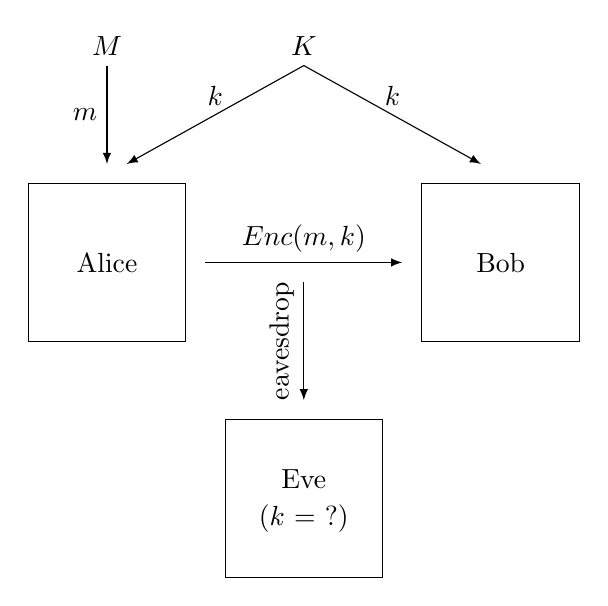
\begin{tikzpicture}
\draw (0,0) rectangle (2,2);
\draw[-latex] (2.25,1) -- (4.75,1);
\draw (5,0) rectangle (7,2);
\node at (1,1) {Alice};
\node at (6,1) {Bob};
\node[anchor=south] at (3.5,1) {$Enc(m,k)$};

\draw[-latex] (1,3.5) -- (1,2.25);
\node[anchor=east] at (1,2.875) {$m$};
\node[anchor=south] at (1,3.5) {$M$};

\node[anchor=south] at (3.5,3.5) {$K$};
\draw[-latex] (3.5,3.5) -- (1.25,2.25);
\draw[-latex] (3.5,3.5) -- (5.75,2.25);
\node[anchor=south] at (2.375,2.875) {$k$};
\node[anchor=south] at (4.625,2.875) {$k$};

\draw (2.5,-3) rectangle (4.5,-1);
\node at (3.5,-1.75) {Eve};
\node at (3.5,-2.25) {($k$ = ?)};
\draw[-latex] (3.5,0.75) -- (3.5,-0.75);
\node[anchor=south,rotate=90] at (3.5,0) {eavesdrop};
\end{tikzpicture}
\end{center}

\begin{definition}[Encryption scheme]
An encryption scheme for (the message) $M$ consists of a key $K$ and a ciphertext $C = Enc(M,K)$, such that
\begin{itemize}
\item $I(M;K) = 0$ (the key is independent of the message -- this is a \term{setup assumption})
\item $H(M|KC) = 0$ (given the key and the ciphertext, Bob can recover the original message)
\end{itemize}
Note that $M$, $K$ and $C$ are random variables.
\end{definition}
Note that in order to satisfy the second requirement, the encryption function $Enc(\cdot,\cdot)$ needs to be injective: every message is mapped to a \emph{unique} ciphertext. The above definition does not put any constraints on the amount of information that Eve can get from the ciphertext: we still need to explicitly require the scheme to be secure.

\begin{definition}[Perfect security]
An encryption scheme is perfectly secure if
\[
I(M;C) = 0.
\]
This is equivalent to saying $H(M|C) = H(M)$, or to saying that $M$ and $C$ are independent.
\end{definition}
This type of security is also sometimes called perfect \term{information-theoric security}, in order to stress that the ciphertext really does not contain \emph{any} information about the plaintext message. Many commonly used encryption schemes do not provide this type of security. In \term{computationally secure} schemes, a lot of information about the message may be contained in the ciphertext, but it would take a ridiculous amount of resources (such as computation time or memory) to get the information out and derive the message.

Let us consider an example of an perfectly secure scheme:
\begin{example}{One-time pad}
Let $(G,+)$ be some additive group (for example $(\{0,1\}^n, \oplus)$, the group of strings of bits, under bitwise addition modulo 2). If $\mathcal{M} = (G,+)$, define $\mathcal{C} = \mathcal{K} = (G,+)$ and let $K$ be uniformly distributed over all elements of $G$. Then the one-time pad (OTP) is defined by the following encryption and decryption function:
\begin{align*}
Enc(m,k) &= m \oplus k = c,\\
Dec(c,k) &= c \oplus k = m
\end{align*}
For example, if $(G,+) = (\set{0,1}^4,\oplus)$, a possible message $m$ is 0101, and a possible key $k$ is 0110. The ciphertext $c$ is $0101 \oplus 0110 = 0011$, and the decryption of $c$ is again $0011 \oplus 0110 = 0101$, the original message $m$.
\end{example}